\documentclass{standalone}
\usepackage{tikz}

\usetikzlibrary{matrix,positioning,fit}
\usepackage[export]{adjustbox}
\usepackage{tcolorbox}
\usepackage{amsmath}
\usepackage{relsize}

%\tikzset{	font={\fontsize{10pt}{12}\selectfont}}


\begin{document}
	
	
	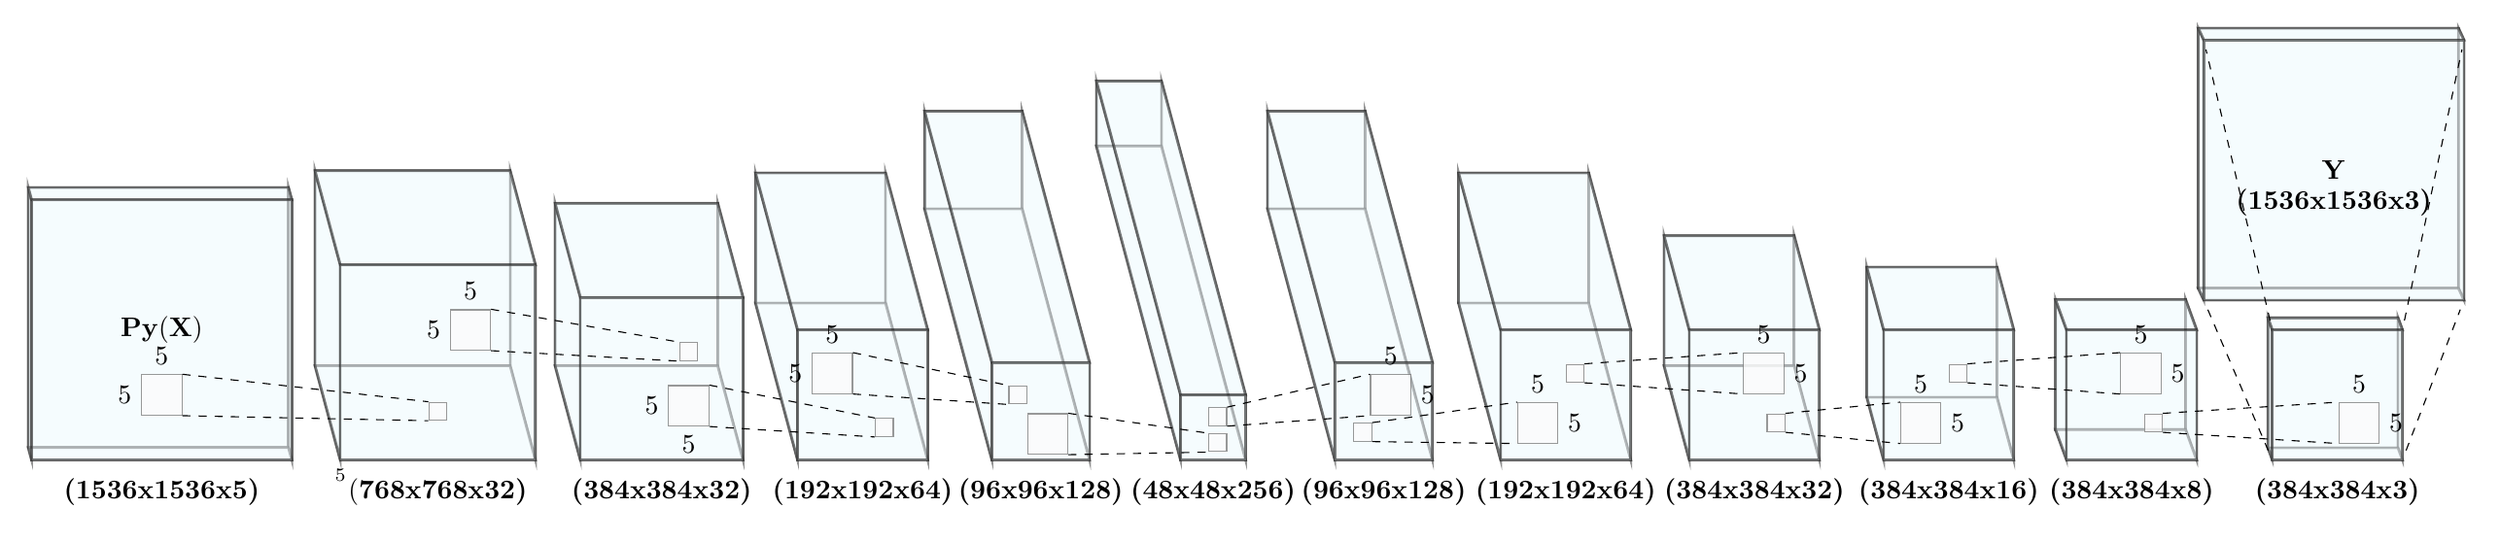
\begin{tikzpicture}[scale=0.85] % le scale permet que le texte soit un peu plus gros, car il n'est pas impacté...
	\newlength{\hofsg}
	\settoheight{\hofsg}{}  

%    \tikzstyle{every node}=[line width=]


	
	
	\newcommand{\drawcube}[5]{
		\pgfmathsetmacro{\Theta}{90+#4}
		\pgfmathsetmacro{\Width}{#1}
		\pgfmathsetmacro{\Height}{#2}
		\pgfmathsetmacro{\Depth}{#3}
		\pgfmathsetmacro{\Opacity}{#5}
		
		
		\pgfmathsetmacro{\Dey}{sin(\Theta)*\Depth}
		\pgfmathsetmacro{\Dex}{cos(\Theta)*\Depth}
		
		\coordinate (A) at (0,0,0);
		\coordinate (B) at (0,\Height,0);
		\coordinate (C) at (\Width,\Height,0);
		\coordinate (D) at (\Width,0,0);
		
		\coordinate (E) at (\Dex,\Dey);
		\coordinate (F) at (\Dex,\Height+\Dey);
		\coordinate (G) at (\Width+\Dex,\Height+\Dey);
		\coordinate (H) at (\Width+\Dex,0+\Dey);
		
		\draw[black!85,fill=cyan!5,opacity=\Opacity, line width=1] (E) -- (F) -- (G) -- (H) -- cycle;% Back Face
		\draw[black!85,fill=cyan!5,opacity=\Opacity, line width=1] (D) -- (C) -- (G) -- (H) -- cycle;% Left Face
		\draw[black!85,fill=cyan!5,opacity=\Opacity, line width=1] (A) -- (D) -- (H) -- (E) -- cycle;% Bottom Face
		\draw[black!85,fill=cyan!5,opacity=\Opacity, line width=1] (A) -- (B) -- (F) -- (E) -- cycle;% Right Face
		\draw[black!85,fill=cyan!5,opacity=\Opacity, line width=1] (B) -- (C) -- (G) -- (F) -- cycle;% Top Face
		\draw[black!85,fill=cyan!5,opacity=\Opacity, line width=1] (A) -- (B) -- (C) -- (D) -- cycle;% Front Face   
	}
	
	\newcommand{\drawsmallcube}[9]{
		\pgfmathsetmacro{\Theta}{90+#4}
		\pgfmathsetmacro{\Width}{#1}
		\pgfmathsetmacro{\Height}{#2}
		\pgfmathsetmacro{\Depth}{#3}
		\pgfmathsetmacro{\Opacity}{#5}
		\pgfmathsetmacro{\x}{#6}
		\pgfmathsetmacro{\y}{#7}
		\pgfmathsetmacro{\lx}{#8}
		\pgfmathsetmacro{\ly}{#9}
		\pgfmathsetmacro{\name}{#10}
		
		\pgfmathsetmacro{\Dey}{sin(\Theta)*\Depth}
		\pgfmathsetmacro{\Dex}{cos(\Theta)*\Depth}
		
		\coordinate (A) at (\x,\y,0);
		\coordinate (B) at (\x,\y+\Height,0);
		\coordinate (C) at (\x+\Width,\y+\Height,0);
		\coordinate (D) at (\x+\Width,\y,0);
		
		\coordinate (E) at (\x+\Dex,\y+\Dey);
		\coordinate (F) at (\x+\Dex,\y+\Height+\Dey);
		\coordinate (G) at (\x+\Width+\Dex,\y+\Height+\Dey);
		\coordinate (H) at (\x+\Width+\Dex,\y+\Dey);
		
		\draw[gray,fill=black!5,opacity=\Opacity] (E) -- (F) -- (G) -- (H) -- cycle;% Back Face
		\draw[gray,fill=black!5,opacity=\Opacity] (D) -- (C) -- (G) -- (H) -- cycle;% Left Face
		\draw[gray,fill=black!5,opacity=\Opacity] (A) -- (D) -- (H) -- (E) -- cycle;% Bottom Face
		\draw[gray,fill=black!5,opacity=\Opacity] (A) -- (B) -- (F) -- (E) -- cycle;% Right Face
		\draw[gray,fill=black!5,opacity=\Opacity] (B) -- (C) -- (G) -- (F) -- cycle;% Top Face
		\draw[gray,fill=black!5,opacity=\Opacity, name=\name, label=north:\lx, label=west:\ly] (A) -- (B) -- (C) -- (D) -- cycle;% Front Face   
	}
	
	
	
	
	
	\pgfmathsetmacro{\feata}{4}%512
	\pgfmathsetmacro{\featb}{3}%256
	\pgfmathsetmacro{\featc}{2.5}%128
	\pgfmathsetmacro{\featd}{2}%64
	\pgfmathsetmacro{\feate}{1.5}%32
	\pgfmathsetmacro{\featf}{1}%32
	\pgfmathsetmacro{\featg}{1.5}%32
	\pgfmathsetmacro{\feath}{2}%32
	\pgfmathsetmacro{\feati}{2}%32
	\pgfmathsetmacro{\featj}{2}%32
	\pgfmathsetmacro{\featk}{2}%32
	\pgfmathsetmacro{\featl}{2}%32
	\pgfmathsetmacro{\featm}{4}%32
	
	\pgfmathsetmacro{\pronfa}{0.2}%5
	\pgfmathsetmacro{\pronfb}{1.5}%32
	\pgfmathsetmacro{\pronfc}{1.5}%32
	\pgfmathsetmacro{\pronfd}{2.5}%64
	\pgfmathsetmacro{\pronfe}{4}%128
	\pgfmathsetmacro{\pronff}{5}%256
	\pgfmathsetmacro{\pronfg}{4}%128
	\pgfmathsetmacro{\pronfh}{2.5}%64
	\pgfmathsetmacro{\pronfi}{1.5}%32
	\pgfmathsetmacro{\pronfj}{1}%16
	\pgfmathsetmacro{\pronfk}{0.5}%8
	\pgfmathsetmacro{\pronfl}{0.2}%3
	\pgfmathsetmacro{\pronfm}{0.2}%32
	
	\pgfmathsetmacro{\offseta}{0}%5
	\pgfmathsetmacro{\offsetb}{135}%5
	\pgfmathsetmacro{\offsetc}{240}%5
	\pgfmathsetmacro{\offsetd}{335}%5
	\pgfmathsetmacro{\offsete}{420}%5
	\pgfmathsetmacro{\offsetf}{502.5}%5
	\pgfmathsetmacro{\offsetg}{570}%5
	\pgfmathsetmacro{\offseth}{642.5}%5
	\pgfmathsetmacro{\offseti}{725}%5
	\pgfmathsetmacro{\offsetj}{810}%5
	\pgfmathsetmacro{\offsetk}{890}%5
	\pgfmathsetmacro{\offsetl}{980}%5
	\pgfmathsetmacro{\offsetm}{950}%5
	
	\pgfmathsetmacro{\featang}{25}%4
	\pgfmathsetmacro{\featanga}{15}%4
	\pgfmathsetmacro{\featangb}{15}%4
	\pgfmathsetmacro{\featangc}{15}%4
	\pgfmathsetmacro{\featangd}{15}%4
	\pgfmathsetmacro{\featange}{15}%4
	\pgfmathsetmacro{\featangf}{15}%4
	\pgfmathsetmacro{\featangg}{15}%4
	\pgfmathsetmacro{\featangh}{15}%4
	\pgfmathsetmacro{\featangi}{15}%4
	\pgfmathsetmacro{\featangj}{15}%4
	\pgfmathsetmacro{\featangk}{20}%4
	\pgfmathsetmacro{\featangl}{20}%4
	\pgfmathsetmacro{\featangm}{25}%4
	% \begin{scope}[xshift=0, yshift=150]
	% \drawcube{\fa}{\fa}{0}{30}{0.5}
	% % \node[] at (\fa/2,-0.5) {512};
	% % \node[] at (-0.5,\fa/2) {512};
	% \node[] at (\fa/2,\fa/2) {$X$};
	% \node[] at (\fa/2,\fa+0.5) {(512x512)};
	% \end{scope}   
	
	\begin{scope}[xshift=\offseta, yshift=0]
	\drawcube{\feata}{\feata}{\pronfa}{\featanga}{0.5}
	% \node[] at (\fa/2,-0.5) {512};
	% \node[] at (-0.5,\fa/2) {512};
	% \node[] at (0,\fa+0.5) {4};
	\node[] at (\feata/2,-0.5) {\textbf{(1536x1536x5)}};
	\node[] at (\feata/2,\feata/2) {$\mathbf{Py(X)}$};
	\node at (\feata/2,\feata/4) [draw,gray, fill=black!1,opacity=0.8, name=rect11, rectangle, minimum width=15,minimum height=15, label=north:5, label=west:5] {};
	%\drawsmallcube{0.5}{0.5}{\pronff}{30}{0.5}{1.75}{1.75}{5}{5}{rect304}
	\end{scope}   
	
	%\begin{scope}[xshift=300, yshift=0]
	%\drawcube{4}{4}{0.8}{30}{0.5}
	%\node[] at (1,-0.5) {512};
	%\node[] at (-0.5,1) {512};
	%\node[] at (0.,4.5) {32};
	%\end{scope}   
	
	\begin{scope}[xshift=\offsetb, yshift=0]
	\drawcube{\featb}{\featb}{\pronfb}{\featangb}{0.5}
	% \node[] at (\fb/2,-0.5) {256};
	% \node[] at (-0.5,\fb/2) {256};
	% \node[] at (0.,\fb+0.5) {32};
	\node[] at (\featb/2,-0.5) {(\textbf{768x768x32)}};
	
	\node at (\featb/2,\featb/4) [draw, gray,fill=black!1,opacity=0.8, name=rect12, rectangle, minimum width=1,minimum height=1] {};
	
	\node at (\feata/2,\feata/2) [draw, gray,fill=black!1,opacity=0.8, name=rect21, rectangle, minimum width=15,minimum height=15, label=north:5, label=west:5] {} node[draw=none,fill=none,font=\scriptsize,below] {5};
	
	\end{scope}   
	
	%\draw[] (rect1) -- (rect2) ;
	
	%\begin{scope}[xshift=550, yshift=0]
	%\drawcube{2}{2}{1.6}{30}{0.5}
	%\node[] at (1,-0.5) {256};
	%\node[] at (-0.5,1) {256};
	%\node[] at (0.,2.5) {64};
	%\end{scope}   
	
	
	\begin{scope}[xshift=\offsetc, yshift=0]
	\drawcube{\featc}{\featc}{\pronfc}{\featangc}{0.5}
	% \node[] at (\fc/2,-0.5) {128};
	% \node[] at (-0.5,\fc/2) {128};
	% \node[] at (0.,\fc+.5) {32};
	\node[] at (\featc/2,-0.5) {\textbf{(384x384x32)}};
	\node at (\featc/1.5,\featc/1.5) [draw, gray,fill=black!1,opacity=0.8, name=rect22, rectangle, minimum width=0.1,minimum height=0.1] {};
	\node at (\featc/1.5,\featc/3) [draw, gray, fill=black!1,opacity=0.8, name=rect31, rectangle, minimum width=15,minimum height=15, label=south:5, label=west:5] {};
	\end{scope}   
	
	
	%\begin{scope}[xshift=750, yshift=0]
	%\drawcube{0.5}{0.5}{1.6}{30}{0.5}
	%\node[] at (1,-0.5) {64};
	%\node[] at (-0.5,1) {64};
	%\node[] at (0.,2.5) {64};
	%\end{scope}   
	
	\begin{scope}[xshift=\offsetd, yshift=0]
	\drawcube{\featd}{\featd}{\pronfd}{\featangd}{0.5}
	% \node[] at (\fd/2,-0.5) {64};
	% \node[] at (-0.5,\fd/2) {64};
	% \node[] at (0.,\fd+0.5) {64};
	\node[] at (\featd/2,-0.5) {\textbf{(192x192x64)}};
	
	\node at (\featd/1.5,\featd/4) [draw, gray, fill=black!1,opacity=0.8, name=rect32, rectangle, minimum width=0.01, minimum height=0.01] {};
	\node at (\featd/3.75,\featd/1.5) [draw, gray, fill=black!1,opacity=0.8, name=rect41, rectangle, minimum width=15, minimum height=15, label=north:5, label=west:5] {};
	
	\end{scope}   
	
	
	
	
	%\begin{scope}[xshift=950, yshift=0]
	%\drawcube{0.25}{0.25}{3.2}{30}{0.5}
	%\node[] at (1,-0.5) {32};
	%\node[] at (-0.5,1) {32};
	%\node[] at (0.,2.5) {128};
	%\end{scope}   
	
	\begin{scope}[xshift=\offsete, yshift=0]
	\drawcube{\feate}{\feate}{\pronfe}{\featange}{0.5}
	% \node[] at (\fe/2,-0.5) {32};
	% \node[] at (-0.5,\fe/2) {32};
	% \node[] at (0.,\fe+.5) {128};
	\node[] at (\feate/2,-0.5) {\textbf{(96x96x128)}};
	\node at (\feate/3.75,\feate/1.5) [draw, gray, fill=black!1,opacity=0.8, name=rect42, rectangle, minimum width=0.01,minimum height=0.01] {};
	\node at (\feate/1.75,\feate/3.75) [draw, gray, fill=black!1,opacity=0.8, name=rect51, rectangle, minimum width=15,minimum height=15] {};
	\end{scope}   
	
	
	
	
	\begin{scope}[xshift=\offsetf, yshift=0]
	\drawcube{\featf}{\featf}{\pronff}{\featangf}{0.5}
	% \node[] at (\fd/2,-0.5) {64};
	% \node[] at (-0.5,\fd/2) {64};
	% \node[] at (0.,\fd+.5) {64};
	\node[] at (\featf/2,-0.5) {\textbf{(48x48x256)}};
	\node at (\featf/1.75,\featf/3.75) [draw, gray, fill=black!1,opacity=0.8, name=rect52, rectangle, minimum width=0.01,minimum height=0.01] {};
	\node at (\featf/1.75,\featf/1.5) [draw,gray, fill=black!1,opacity=0.8, name=rect61, rectangle, minimum width=0.01,minimum height=0.01] {};
	\end{scope}
	
	
	\begin{scope}[xshift=\offsetg, yshift=0]
	\drawcube{\featg}{\featg}{\pronfg}{\featangg}{0.5}
	% \node[] at (\fc/2,-0.5) {128};
	% \node[] at (-0.5,\fc/2) {128};
	% \node[] at (0.,\fc+.5) {32};
	\node[] at (\featg/2,-0.5) {\textbf{(96x96x128)}};
	\node at (\featg/1.75,\featg/1.5) [draw, gray, fill=black!1,opacity=0.8, name=rect62, rectangle, minimum width=15,minimum height=15, label=north:5, label=east:5] {};
	\node at (\featg/3.5,\featg/3.5) [draw, gray, fill=black!1,opacity=0.8, name=rect71, rectangle, minimum width=0.01,minimum height=0.01] {};
	\end{scope}    
	
	
	
	
	\begin{scope}[xshift=\offseth, yshift=0]
	\drawcube{\feath}{\feath}{\pronfh}{\featangh}{0.5}
	% \node[] at (\fc/2,-0.5) {128};
	% \node[] at (-0.5,\fc/2) {128};
	% \node[] at (0.,\fc+.5) {16};
	\node[] at (\feath/2,-0.5) {\textbf{(192x192x64)}};
	\node at (\feath/3.5,\feath/3.5) [draw, gray, fill=black!1,opacity=0.8, name=rect72, rectangle, minimum width=15,minimum height=15, label=north:5, label=east:5] {};
	\node at (\feath/1.75,\feath/1.5) [draw, gray, fill=black!1,opacity=0.8, name=rect81, rectangle, minimum width=0.01,minimum height=0.01] {};
	\end{scope}  
	
	
	
	\begin{scope}[xshift=\offseti, yshift=0]
	\drawcube{\feati}{\feati}{\pronfi}{\featangi}{0.5}
	% \node[] at (\fc/2,-0.5) {128};
	% \node[] at (-0.5,\fc/2) {128};
	% \node[] at (0.,\fc+.5) {8};
	\node[] at (\feati/2,-0.5) {\textbf{(384x384x32)}};
	\node at (\feati/1.75,\feati/1.5) [draw, gray, fill=black!1,opacity=0.8, name=rect82, rectangle, minimum width=15,minimum height=15, label=north:5, label=east:5] {};
	\node at (\feati/1.5,\feati/3.5) [draw, gray, fill=black!1,opacity=0.8, name=rect91, rectangle, minimum width=0.01,minimum height=0.01] {};
	\end{scope}
	
	
	
	\begin{scope}[xshift=\offsetj, yshift=0]
	\drawcube{\featj}{\featj}{\pronfj}{\featangj}{0.5}
	% \node[] at (\fc/2,\fc+0.5) {128};
	% \node[] at (\fc+0.5,\fc/2) {128};
	\node[] at (\featj/2,-0.5) {\textbf{(384x384x16)}};
	\node[name=beg1] at (0,0) {};
	\node[name=beg2] at (\featj,0) {};
	\node[name=beg3] at (0,\featj) {};
	\node[name=beg4] at (\featj,\featj) {};
	\node at (\featj/3.5,\featj/3.5) [draw, gray, fill=black!1,opacity=0.8, name=rect92, rectangle, minimum width=15,minimum height=15, label=north:5, label=east:5] {};
	\node at (\featj/1.75,\featj/1.5) [draw, gray, fill=black!1,opacity=0.8, name=rect101, rectangle, minimum width=0.01,minimum height=0.01] {};
	\end{scope}
	
	
	
	
	\begin{scope}[xshift=\offsetk, yshift=0]
	\drawcube{\featk}{\featk}{\pronfk}{\featangk}{0.5}
	% \node[] at (\fc/2,\fc+0.5) {128};
	% \node[] at (\fc+0.5,\fc/2) {128};
	\node[] at (\featk/2,-0.5) {\textbf{(384x384x8)}};
	\node[name=beg1] at (0,0) {};
	\node[name=beg2] at (\featk,0) {};
	\node[name=beg3] at (0,\featk) {};
	\node[name=beg4] at (\featk,\featk) {};
	\node at (\featk/1.75,\featk/1.5) [draw, gray, fill=black!1,opacity=0.8, name=rect102, rectangle, minimum width=15,minimum height=15, label=north:5, label=east:5] {};
	\node at (\featk/1.5,\featk/3.5) [draw, gray, fill=black!1,opacity=0.8, name=rect111, rectangle, minimum width=0.01,minimum height=0.01] {};
	\end{scope}
	
	
	
	\begin{scope}[xshift=\offsetl, yshift=0]
	\drawcube{\featl}{\featl}{\pronfl}{\featangl}{0.5}
	% \node[] at (\fc/2,\fc+0.5) {128};
	% \node[] at (\fc+0.5,\fc/2) {128};
	\node[] at (\featl/2,-0.5) {\textbf{(384x384x3)}};
	\node[name=beg1] at (0,0) {};
	\node[name=beg2] at (\featl,0) {};
	\node[name=beg3] at (0,\featl) {};
	\node[name=beg4] at (\featl,\featl) {};
	\node at (\featl/1.5,\featl/3.5) [draw, gray, fill=black!1,opacity=0.8, name=rect112, rectangle, minimum width=15,minimum height=15, label=north:5, label=east:5] {};
	\end{scope}
	
	
	\draw[dashed] (rect11.north east) -- (rect12.north west);
	\draw[dashed] (rect11.south east) -- (rect12.south west);
	\draw[dashed] (rect21.north east) -- (rect22.north west);
	\draw[dashed] (rect21.south east) -- (rect22.south west);
	\draw[dashed] (rect31.north east) -- (rect32.north west);
	\draw[dashed] (rect31.south east) -- (rect32.south west);
	\draw[dashed] (rect41.north east) -- (rect42.north west);
	\draw[dashed] (rect41.south east) -- (rect42.south west);
	\draw[dashed] (rect51.north east) -- (rect52.north west);
	\draw[dashed] (rect51.south east) -- (rect52.south west);
	\draw[dashed] (rect61.north east) -- (rect62.north west);
	\draw[dashed] (rect61.south east) -- (rect62.south west);
	\draw[dashed] (rect71.north east) -- (rect72.north west);
	\draw[dashed] (rect71.south east) -- (rect72.south west);
	\draw[dashed] (rect81.north east) -- (rect82.north west);
	\draw[dashed] (rect81.south east) -- (rect82.south west);
	\draw[dashed] (rect91.north east) -- (rect92.north west);
	\draw[dashed] (rect91.south east) -- (rect92.south west);
	\draw[dashed] (rect101.north east) -- (rect102.north west);
	\draw[dashed] (rect101.south east) -- (rect102.south west);
	\draw[dashed] (rect111.north east) -- (rect112.north west);
	\draw[dashed] (rect111.south east) -- (rect112.south west);
	
	\begin{scope}[xshift=\offsetm, yshift=70]
	\drawcube{\featm}{\featm}{\pronfm}{\featangm}{0.5}
	% \node[] at (\fa/2,\fa+0.5) {512};
	% \node[] at (-0.5,\fa/2) {512};
	\node[] at (\featm/2,\featm/2-0.5) {\textbf{(1536x1536x3)}};
	\node[name=end1] at (0,0) {};
	\node[name=end2] at (\featm,0) {};
	\node[name=end3] at (0,\featm) {};
	\node[name=end4] at (\featm,\featm) {};
	\node[] at (\featm/2,\featm/2) {$\mathbf{Y}$};
	\end{scope}
	
	\draw[dashed] (beg1) -- (end1);
	\draw[dashed] (beg2) -- (end2);
	\draw[dashed] (beg3) -- (end3);
	\draw[dashed] (beg4) -- (end4);
	
	
	\end{tikzpicture}
	

	
	
\end{document}